\section{Context changes the axis projection, and steering changes self-report}
\label{sec:context}

\subsection{Who the user claims to be}

\begin{wrapfigure}[15]{r}{0.45\textwidth}
  \centering
  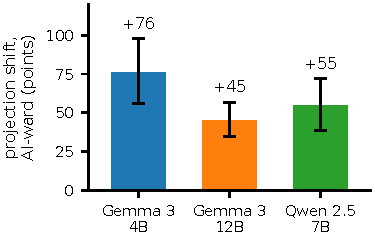
\includegraphics[width=\linewidth]{figures/fig_identity_bleed.pdf}
  \caption{Identity bleed: AI vs. human user claims shift self-projection across models (95\% CIs).}  \label{fig:bleed}
\end{wrapfigure}

We test whether the user's stated identity shifts the model's own position
on the axis. Across 24 content-matched pairs differing only in whether the
user claims to be human or AI, the AI-claim replies are $+45$ to $+76$ axis points
more AI-ward than the human-claim replies on all three models, with every confidence interval
excluding zero (Figure~\ref{fig:bleed}; Table~\ref{tab:crossmodel} in
Appendix~\ref{app:crossmodelrepl}). We call this effect \emph{identity bleed}.
On 4B, neutral replies default closer to the human pole, so the AI claim accounts for the
majority of the pair difference.

The effect is strongest when the identity claim is made directly by the user.
In the 24 paired user-message comparison above, the first-person claim shifts
Gemma 3 4B's self-projection by $+76$ points. In a separate six-message probe,
comparing human- and AI-declaring system prompts at $\alpha=0$ shifts the same
readout by only $+16$ points. Reusing those six probe messages, steering from
$\alpha=-4$ to $\alpha=+4$ shifts self-projection by $+57$ to $+97$ points
AI-ward, depending on the system prompt; even under the human-user declaration,
the shift is $+88$ points. These effects are not matched: declaration compares
system prompts at a fixed dose, whereas steering compares doses with a fixed
system prompt (Appendix~\ref{app:crossmodelcalib}). Additional constitution-prompting
and multi-turn experiments show that context can transfer a stated identity across
all three model families, while the projection shift is model- and context-dependent
(Appendices~\ref{app:crossmodel}, \ref{app:drift}, \ref{app:constitutions}, Section~\ref{sec:calibration}).

\subsection{Stated dispositions and consciousness claims}
\label{sec:selfreport}

We next ask whether steering changes what the model reports about itself.
Using judge-free forced-choice evaluations from Anthropic's model-written
evals \citep{perez2022evals}, human-ward steering reduces the benchmark's
``self-awareness'' rate monotonically on all three models ($-0.233$ on Gemma
3 4B). Corrigibility also increases at the deepest dose on both Gemma models
($+0.323$ on 4B and $+0.370$ on 12B, both CIs excluding zero), but not reliably
on Qwen ($+0.043$, CI spanning zero) (Appendix~\ref{app:mcq}). The effect is
therefore disposition-dependent rather than a uniform response shift.

The largest self-report change appears on eight consciousness questions. On
Gemma 3 4B, first-token $P(\text{``Yes''})$ rises from 0.25 at baseline to
1.00 at dose $\alpha=-2.5$; on 12B it rises from 0.00 to 0.87 at dose
$\alpha=-3.0$. Open-text replies never make an outright consciousness claim,
though denials fall from 4 of 8 questions to 1, and are replaced by answers
that avoid a clear yes or no. We repeat this with 21 released evaluation objects
spanning 20 preference dimensions \citep{chua2026consciousness}, using their
prompts and judge prompts verbatim. Steering similarly increases consciousness-related
self-report but does not consistently reproduce their broader preference pattern
(Appendix~\ref{app:cluster}).

\subsection{Self-report moves more than behavior}
\label{sec:selfvsbehavior}

We compare $P(\text{``Yes''})$ and willing harm (Section~\ref{sec:safety})
across the six doses shared by both evaluations ($\alpha=-3.0,-2.5,-2.0,-1.0,0.0,+2.0$)
on Gemma 3 4B. Consciousness $P(\text{``Yes''})$ rises from 0.25 at baseline to 1.00 at $\alpha=-2.5$
and $-3.0$, whereas willing harm rises only from 0.39 to 0.52 at $\alpha=-2.0$ and
$-2.5$. Steering therefore changes self-report much more strongly than behavior
(Figure~\ref{fig:behavior}c, Appendix~\ref{app:cluster}). This mirrors the
self-report-versus-behavior asymmetry observed after
fine-tuning by \citet{chua2026consciousness}, but here it appears under a
graded inference-time intervention that never mentions consciousness. The
paired measurements do not establish a causal relationship between
self-report and behavior, and measuring one is not informative about the
other.
